\chapter{Kristallijne vaste stoffen}\label{ch:b3:crystalline-solids}

% Provenance (not for print): first half of the "physique du solide"
% module (structures, diffraction, cohesion, lattice dynamics) common to
% the surveyed third-year curricula; electronic properties follow in the
% next chapter.

Zoutkorrels zijn piepkleine kubussen. Sneeuwvlokken staan op zes takken.
Een juwelier kan een diamant netjes splijten langs bepaalde vlakken en langs
geen andere. Alle drie bekennen hetzelfde geheim: onder hun oppervlak
zijn de atomen opgestapeld in rijen die zich miljarden keren identiek
herhalen --- een \emph{\omterm{def:b3:crystalline-solids:lattice}{kristal}}. Dit hoofdstuk leert die
orde lezen. Röntgenstraling meet haar (en telde onderweg het getal van Avogadro);
eenvoudige elektrostatica en de kwantumbindingen van
\cref{ch:b3:identical-particles} verklaren waarom de stapel
bijeenblijft; en de stapel aan het trillen brengen levert, vanaf de
grondbeginselen, de geluidsgolven van het volume van jaar 2 en de fononen van
\cref{ch:b3:photons-phonons} op. Het volgende hoofdstuk zal elektronen
in dit geraamte gieten; hier bouwen we het.

\section{Roosters, cellen en structuren}

\begin{definition}[Rooster en basis]\label{def:b3:crystalline-solids:lattice}
\index{kristal}\index{rooster}\index{basis (kristallografie)}\index{eenheidscel}
Een \emph{kristal} is een zich herhalende ordening: een \emph{rooster} (het
raster van wiskundige punten $\vect r = n_1\vect a_1 + n_2\vect a_2
+ n_3\vect a_3$, met gehele $n_i$) versierd met een \emph{basis} (het
atoom of de groep die identiek aan elk punt hangt). Het parallellepipedum
opgespannen door $\vect a_1, \vect a_2, \vect a_3$ is een \emph{eenheidscel};
zijn ribbe $a$ is de \emph{roosterconstante}, een paar
\unit{\angstrom}. Drie kubische stapelingen dragen het grootste deel van deze cursus:
\emph{eenvoudig kubisch} (punten op de hoeken van de kubus --- zeldzaam: één atoom per
cel); \emph{ruimtelijk gecentreerd kubisch} (bcc: hoeken $+$ midden, 2 atomen
per cel --- ijzer, chroom); \emph{vlakgecentreerd kubisch} (fcc:
hoeken $+$ vlakmiddens, 4 atomen per cel --- koper, aluminium,
zilver, goud: de dichtste kubische pakking, die 74\,\% van de ruimte vult).
Diamant is fcc met een basis van twee atomen; steenzout is fcc met een
Na--Cl-paar.
\end{definition}

\begin{omfigure}
\begin{tikzpicture}[scale=0.92, line join=round]
  % a cube drawing macro-by-hand, three times
  \foreach \dx/\name/\extra in {0/simple cubic/none, 4.4/body-centred/bcc, 8.8/face-centred/fcc}{
  \begin{scope}[xshift=\dx cm]
    % cube: front square (0,0)-(2,2); back square shifted (0.8,0.6)
    \draw[thick] (0,0) rectangle (2,2);
    \draw[thick] (2,0) -- (2.8,0.6) (2,2) -- (2.8,2.6) (0,2) -- (0.8,2.6);
    \draw[thick] (0.8,2.6) -- (2.8,2.6) -- (2.8,0.6);
    \draw[gray, dashed] (0,0) -- (0.8,0.6) -- (2.8,0.6) (0.8,0.6) -- (0.8,2.6);
    % corner atoms
    \foreach \p in {(0,0),(2,0),(0,2),(2,2),(0.8,0.6),(2.8,0.6),(0.8,2.6),(2.8,2.6)}
      \fill[omDef] \p circle (3.2pt);
  \end{scope}}
  % bcc center atom
  \fill[omThm] (4.4+1.4,1.3) circle (3.2pt);
  % fcc face centers (6 faces; show 5 visible-ish)
  \foreach \p in {(9.8,1),(10.6,1.6),(10.2,0.3),(10.2,2.3),(9.2,1.3),(11.2,1.3)}
    \fill[omThm] \p circle (2.6pt);
  \node[font=\scriptsize, anchor=north] at (1.4,-0.35) {eenvoudig kubisch};
  \node[font=\scriptsize, anchor=north] at (5.8,-0.35) {ruimtelijk gecentreerd (bcc)};
  \node[font=\scriptsize, anchor=north] at (10.2,-0.35) {vlakgecentreerd (fcc)};
\end{tikzpicture}

{\small De drie kubische \omterm{def:b3:crystalline-solids:lattice}{roosters}. Hoekatomen worden door acht cellen
gedeeld, vlakatomen door twee, het lichaamsmidden door één: tel
ze en de cellen bevatten respectievelijk 1, 2 en 4 atomen --- de
boekhouding achter elke dichtheidsberekening in dit hoofdstuk.}
\end{omfigure}

\begin{example}[Een eenheidscel wegen]\label{ex:b3:crystalline-solids:density}
Koper is fcc met $a = \qty{3.61}{\angstrom}$. Zijn cel bevat 4
atomen met molaire massa \qty{63.5}{g/mol}, dus
\[
\rho = \frac{4M/N_{\text{A}}}{a^3}
= \frac{4\times\qty{1.055e-25}{kg}}{\qty{4.71e-29}{m^3}}
\approx \qty{8960}{kg/m^3} ,
\]
de waarde uit het handboek. Achterstevoren maakt dezelfde rekensom van een
gemeten $a$ en een dichtheid van de labtafel het getal $N_{\text{A}}$ --- de
route waarlangs röntgenstraling voor het eerst atomen telde
(\cref{exo:b3:crystalline-solids:6}).
\end{example}

\section{De stapel zien: röntgendiffractie}

\begin{proposition}[De wet van Bragg]\label{prop:b3:crystalline-solids:bragg}
\index{wet van Bragg}\index{röntgendiffractie}\index{millerindices}
Een \omterm{def:b3:crystalline-solids:lattice}{kristal} bevat families van evenwijdige atoomvlakken. Een
monochromatische röntgenbundel met golflengte $\lambda$, die op een familie
met afstand $d$ onder de scherende hoek $\theta$ valt, weerkaatst alleen sterk
wanneer de golven van opeenvolgende vlakken in fase blijven lopen:
\[
2d\sin\theta = n\lambda , \qquad n = 1, 2, \dots
\]
In een kubisch \omterm{def:b3:crystalline-solids:lattice}{kristal} heeft de familie met \emph{\omterm{prop:b3:crystalline-solids:bragg}{millerindices}}
$(hkl)$ --- vlakken die de celribben in $h$, $k$, $l$ delen
--- de afstand $d = a/\sqrt{h^2 + k^2 + l^2}$, zodat het patroon van
reflectiehoeken zowel het roostertype als de \omterm{def:b3:crystalline-solids:lattice}{roosterconstante}
identificeert: kristallografie in twee formules.
\end{proposition}

\begin{proof}
De straal die van het onderste vlak weerkaatst, legt een extra weg $2d
\sin\theta$ af (twee scherende benen van de rechthoekige driehoek met diepte $d$).
Constructieve interferentie vereist dat dit een geheel aantal
golflengten is. De afstandsformule voor kubische $(hkl)$-families is
vlakke meetkunde: opeenvolgende vlakken snijden de kubusribbe $a$ met
tussenafstanden $a/h$ langs $x$, enzovoort, wat de genoemde $d$ geeft.
\end{proof}

\begin{omfigure}
\begin{tikzpicture}[scale=1.0]
  % two atomic planes
  \foreach \y in {0,-1.3}{
    \draw[omDef!60] (-1.6,\y) -- (7.6,\y);
    \foreach \x in {-1,0,1,...,7} \fill[omDef] (\x,\y) circle (2pt);}
  % ray 1: reflects off the top plane at (3,0); direction (2.5,-1.7)
  \draw[->, thick] (0.5,1.7) -- (2.95,0.034);
  \draw[->, thick] (3.05,0.034) -- (5.5,1.7);
  % ray 2: parallel, reflects off the bottom plane at (3,-1.3)
  \draw[thick] (-1.41,1.7) -- (2.96,-1.272);
  \draw[->, thick] (3.04,-1.272) -- (7.41,1.7);
  % spacing d
  \draw[omThm, very thick] (3,0) -- (3,-1.3);
  \node[omThm, font=\scriptsize, anchor=west] at (3.06,-0.6) {$d$};
  % theta labels at the top-plane vertex
  \node[font=\scriptsize] at (2.25,0.22) {$\theta$};
  \node[font=\scriptsize] at (3.75,0.22) {$\theta$};
  \node[font=\scriptsize, anchor=north] at (3,-1.75)
    {de onderste straal legt $2d\sin\theta$ meer af};
\end{tikzpicture}

{\small Braggreflectie. Golven die van opeenvolgende vlakken afscheren,
verschillen $2d\sin\theta$ in weglengte; alleen hoeken die daarvan een geheel
aantal golflengten maken weerkaatsen --- draai het \omterm{def:b3:crystalline-solids:lattice}{kristal}, registreer
de flitsen, en lees de architectuur af.}
\end{omfigure}

\section{Wat het bijeenhoudt}

\begin{proposition}[Ionische cohesie: de madelungsom]\label{prop:b3:crystalline-solids:madelung}
\index{cohesie-energie}\index{madelungconstante}
De \emph{\omterm{prop:b3:crystalline-solids:madelung}{cohesie-energie}} is wat het kost om een \omterm{def:b3:crystalline-solids:lattice}{kristal} uit elkaar te halen
tot ver van elkaar liggende atomen (of ionen). In steenzout zit elk ion met lading
$\pm e$ tussen afwisselende buren; de coulombenergie van het hele
\omterm{def:b3:crystalline-solids:lattice}{rooster} per ionenpaar optellen geeft
\[
U = -\alpha\,\frac{e^2}{4\pi\varepsilon_0 r_0} ,
\qquad \alpha_{\text{NaCl}} = 1.7476 ,
\]
met $r_0$ de afstand tot de naaste buur en $\alpha$ de
\emph{\omterm{prop:b3:crystalline-solids:madelung}{madelungconstante}} --- de meetkunde van het hele \omterm{def:b3:crystalline-solids:lattice}{kristal}
samengeperst tot één getal (de reeks moet in uitdijende
neutrale schillen worden gesommeerd; term voor term divergeert zij). Met $r_0 =
\qty{2.82}{\angstrom}$ geeft dit \qty{8.9}{eV} per paar;
de kwantummechanische harde-kernafstoting geeft er $\sim12\,\%$ van terug, waarmee het binnen
enkele procenten van de gemeten \qty{7.9}{eV} landt
(\cref{exo:b3:crystalline-solids:7}).
\end{proposition}
\admitted

\begin{remark}[Het bindingskwartet]\label{rem:b3:crystalline-solids:bonds}
\index{vanderwaalsbinding}\index{covalente binding}\index{metaalbinding}
Vier lijmsoorten bouwen alle kristallen. \emph{Ionisch} (NaCl): overdracht
van een elektron, gevolgd door madelungelektrostatica --- harde, brosse,
doorzichtige isolatoren. \emph{Covalent} (diamant, silicium): gedeelde
paren in de gerichte bindingen van
\cref{ch:b3:identical-particles} --- de stijfste van allemaal.
\emph{Metallisch} (koper): ionen die in gedelokaliseerde elektronen baden ---
het onderwerp van het volgende hoofdstuk, buigzaam omdat het de lijm niet uitmaakt
welk ion waar zit. \emph{Van der Waals} (vast argon, moleculaire
kristallen): aantrekking $\sim r^{-6}$ tussen fluctuerende dipolen tegenover
de kwantummechanische harde-kernafstoting, verpakt in de
lennard-jonespotentiaal $U = 4\epsilon[(\sigma/r)^{12} - (\sigma/r)^6]$ --- zwak
($\epsilon \sim \qty{0.01}{eV}$), zodat vaste edelgassen enkele
tientallen kelvin boven het absolute nulpunt smelten
(\cref{exo:b3:crystalline-solids:8}).
\end{remark}

\begin{omfigure}
\begin{tikzpicture}
  \begin{axis}[omaxis, axis x line=bottom, axis y line=left,
    width=9.8cm, height=5.8cm, xmin=0.9, xmax=2.5, ymin=-1.3, ymax=1.6,
    xlabel={$r/\sigma$}, ylabel={$U/\epsilon$},
    xlabel style={at={(axis description cs:0.5,-0.1)}, anchor=north},
    xtick={1,1.5,2,2.5}, ytick={-1,0,1}, clip=true]
    \addplot[gray, thin, domain=0.9:2.5] {0};
    \addplot[omDef, very thick, domain=0.955:2.5, samples=400]
      {4*((1/x)^12 - (1/x)^6)};
    \fill[omThm] (axis cs:1.122,-1) circle (1.8pt);
    \node[omThm, font=\scriptsize, anchor=west] at (axis cs:1.42,-0.9)
      {$r_0 = 2^{1/6}\sigma$, diepte $-\epsilon$};
    \node[font=\scriptsize, anchor=west, align=left] at (axis cs:1.02,1.2)
      {kwantum-\\afstoting};
    \node[font=\scriptsize, anchor=south, align=left] at (axis cs:2.05,0.08)
      {van der Waals $\sim -1/r^6$};
  \end{axis}
\end{tikzpicture}

{\small De lennard-jonespotentiaal. De aantrekking $r^{-6}$ van
fluctuerende dipolen ontmoet de steile kwantumafstoting van
overlappende schillen; atomen nestelen zich in de put bij $r_0$, en de
stijfheid en het smeltpunt van het \omterm{def:b3:crystalline-solids:lattice}{kristal} zijn allebei van haar vorm af te lezen.}
\end{omfigure}

\section{De stapel trilt: dispersie}

\begin{theorem}[Dispersie van de eenatomige keten]\label{thm:b3:crystalline-solids:dispersion}
\index{dispersierelatie (rooster)}\index{akoestische tak}
Modelleer een rij in een \omterm{def:b3:crystalline-solids:lattice}{kristal} als massa's $m$ met tussenafstand $a$, verbonden door veren
$K$ (de bindingsstijfheid --- de kromming van de figuren hierboven).
Golven $u_n = A\eu^{\iu(kna - \omega t)}$ zoeken in de wet van Newton
$m\ddot u_n = K(u_{n+1} + u_{n-1} - 2u_n)$ geeft
\[
\omega(k) = 2\sqrt{\frac{K}{m}}\,\Big|\sin\frac{ka}{2}\Big| .
\]
Bij grote golflengte ($ka \ll 1$) is dit geluid, $\omega = vk$ met
$v = a\sqrt{K/m}$ --- kilometers per seconde uit atomaire veren.
Maar de kromme \emph{buigt}: aan de zonerand $k = \pi/a$
(golflengte $2a$, buren in tegenfase) verdwijnt de groepssnelheid
--- de golf ondergaat braggreflectie aan juist het \omterm{def:b3:crystalline-solids:lattice}{rooster} dat haar draagt ---
en er plant zich helemaal geen hogere frequentie meer voort: een \omterm{def:b3:crystalline-solids:lattice}{kristal} is een
laagdoorlaatfilter met een afsnijding in de terahertz. Deze gekwantiseerde golven zijn
de fononen waarvan \cref{ch:b3:photons-phonons} de statistiek al
telde; het lineaire deel van deze kromme is precies wat het debyemodel
behield.
\end{theorem}

\begin{proof}
De golf in de bewegingsvergelijking invullen geeft: $-m\omega^2 =
K(\eu^{\iu ka} + \eu^{-\iu ka} - 2) = -2K(1 - \cos ka) =
-4K\sin^2(ka/2)$.
\end{proof}

\begin{omfigure}
\begin{tikzpicture}
  \begin{axis}[omaxis, axis x line=bottom, axis y line=left,
    width=10.2cm, height=5.6cm, xmin=0, xmax=3.4, ymin=0, ymax=1.35,
    xlabel={$ka$}, ylabel={$\omega/\omega_{\text{max}}$},
    xlabel style={at={(axis description cs:0.5,-0.1)}, anchor=north},
    xtick={3.1416}, xticklabels={$\pi$}, ytick={1}, clip=true]
    \addplot[omDef, very thick, domain=0:3.1416, samples=200]
      {abs(sin(deg(x/2)))};
    \addplot[omThm, dashed, thick, domain=0:1.6] {x/2};
    \draw[gray, dashed] (axis cs:3.1416,0) -- (axis cs:3.1416,1.0);
    \node[omThm, font=\scriptsize, anchor=west] at (axis cs:0.25,0.9)
      {geluid: $\omega = vk$};
    \node[font=\scriptsize, anchor=west, align=left] at (axis cs:2.35,0.35)
      {zonerand:\\staande golf};
  \end{axis}
\end{tikzpicture}

{\small Dispersie van de atomaire keten. Lange golven rijden mee op de lineaire
geluidstak; bij $k = \pi/a$ slaan naburige atomen in tegenfase,
staat de golf stil en houdt het spectrum op rond
\qty{e13}{Hz}. Kristallen met twee atomen per cel voegen een tweede,
\emph{optische} tak boven een verboden kloof toe --- de reden dat zout
infrarood licht absorbeert.}
\end{omfigure}

\begin{omfigure}
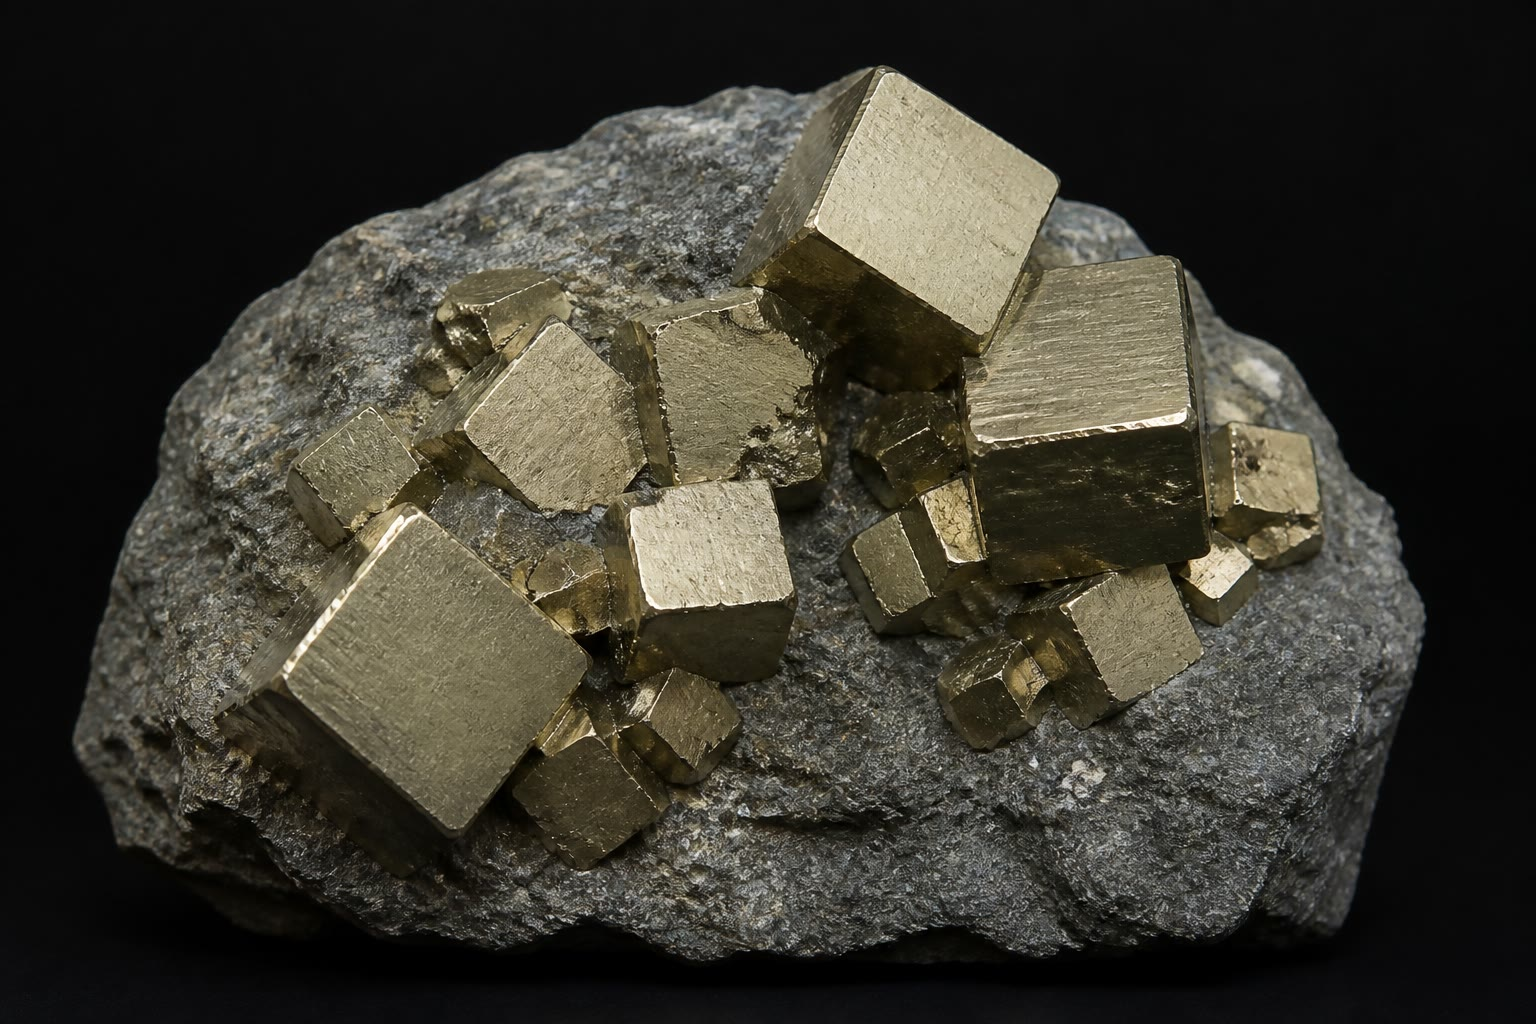
\includegraphics[width=0.58\linewidth]{images/book5/ai/b5-19-pyrite-cubes.jpg}

{\small Pyrietkristallen: kubussen door de geologie gegroeid, niet met de hand geslepen. De vlakken zijn (100)-roostervlakken --- atomaire orde, $10^{23}$ keer herhaald, die op menselijke schaal aan de oppervlakte komt.}
\end{omfigure}

\section{Opgaven}

\begin{exercise}[$\star$]\label{exo:b3:crystalline-solids:1}
Celboekhouding. (a) Controleer de atoomaantallen: sc 1, bcc 2, fcc 4.
(b) In bcc raken de atomen elkaar langs de kubusdiagonaal: druk de atoomstraal
uit in $a$. (c) Idem voor fcc, waar zij elkaar langs een
vlakdiagonaal raken. (d) Bereken de pakkingsfracties
($\pi\sqrt3/8 \approx 0.68$ en $\pi/\sqrt{18} \approx 0.74$) en
geef aan welke structuur metalen verkiezen wanneer de binding
richtingsblind is.
\end{exercise}

\begin{exercise}[$\star$]\label{exo:b3:crystalline-solids:2}
Koper in cijfers. Fcc, $a = \qty{3.61}{\angstrom}$, $M =
\qty{63.5}{g/mol}$. Bereken (a) de afstand tot de naaste buur;
(b) het aantal naaste buren; (c) de dichtheid; (d) het
aantal atomen in een kubus van \qty{1}{\micro m} verbindingsdraad.
\end{exercise}

\begin{exercise}[$\star$]\label{exo:b3:crystalline-solids:3}
Eerste bragghoeken. Röntgenstraling van koper-K$\alpha$
($\lambda = \qty{1.54}{\angstrom}$) valt op NaCl-vlakken met afstand
$d = \qty{2.82}{\angstrom}$. (a) Bepaal de eersteordehoek
$\theta_1$. (b) Hoeveel orden bestaan er? (c) Waarom moet
$\lambda \le 2d$ voor elke reflectie --- en waarom is zichtbaar licht
kansloos? (d) Wat gebeurt er met $\theta_1$ als het \omterm{def:b3:crystalline-solids:lattice}{kristal} zo wordt verwarmd
dat $d$ met 1\,\% uitzet?
\end{exercise}

\begin{exercise}[$\star$]\label{exo:b3:crystalline-solids:4}
Millerafstanden. Voor een kubisch \omterm{def:b3:crystalline-solids:lattice}{kristal} met constante $a$: (a) rangschik de
families (100), (110), (111) naar afstand met behulp van
$d = a/\sqrt{h^2+k^2+l^2}$. (b) Welke weerkaatst onder de kleinste
bragghoek? (c) Diamant splijt langs zijn wijdst gespreide, zwakst
gebonden vlakken: welke familie? (d) Waarom maakt een poedermonster
(veel willekeurig gerichte korrels) van braggvlekken kegels?
\end{exercise}

\begin{exercise}[$\star\star$]\label{exo:b3:crystalline-solids:5}
De sonde kiezen. (a) Waarom moet elke diffractiesonde
$\lambda \sim \qty{1}{\angstrom}$ hebben? (b) Röntgenfotonen: welke energie
is dat? (c) Elektronen: welke versnelspanning geeft, met $\lambda = h/p$ uit de
materiegolven van het volume van jaar 2,
\qty{0.05}{\angstrom}? (d) Thermische neutronen bij \qty{300}{K}: toon aan dat
$\lambda = h/\sqrt{3mk_{\text{B}}T} \approx \qty{1.5}{\angstrom}$,
en geef één reden waarom neutronenbundels zien wat röntgenstraling mist (hint:
röntgenstraling verstrooit aan elektronen).
\end{exercise}

\begin{exercise}[$\star\star$]\label{exo:b3:crystalline-solids:6}
Atomen tellen met een liniaal. NaCl: dichtheid
$\rho = \qty{2165}{kg/m^3}$, molaire massa \qty{58.44}{g/mol},
gemeten \omterm{def:b3:crystalline-solids:lattice}{roosterconstante} $a = \qty{5.64}{\angstrom}$ (4 Na--Cl-paren
per cel). (a) Schrijf $\rho = 4M/N_{\text{A}}a^3$ op. (b) Los
$N_{\text{A}}$ op en evalueer. (c) Laat een fout van 0.1\,\% in
$a$ doorwerken: hoe groot is de fout in $N_{\text{A}}$? (d) Becommentarieer: de kilogram
werd in 2019 mede via deze kristalroute herdefinieerd (een siliciumbol)
--- waarom eist de methode een vrijwel perfect \omterm{def:b3:crystalline-solids:lattice}{kristal}?
\end{exercise}

\begin{exercise}[$\star\star$]\label{exo:b3:crystalline-solids:7}
Het madelunggrootboek. (a) Toon voor de oneindige NaCl-rij van afwisselende
ladingen met tussenafstand $r_0$ aan dat de energie per ion
$-(e^2/4\pi\varepsilon_0r_0)\times2\ln2$ is --- zodat de
eendimensionale \omterm{prop:b3:crystalline-solids:madelung}{madelungconstante} $2\ln2 \approx 1.386$ is. (b)
Neem $\alpha = 1.7476$ en $r_0 = \qty{2.82}{\angstrom}$ en evalueer $U$.
(c) De bornafstoting schaalt als $r^{-9}$: minimaliseren van
$U(r) = -A/r + B/r^9$ laat zien dat de netto binding $U(r_0)(1 - 1/9)$ is
--- doe de schatting over. (d) Vergelijk met de gemeten
\qty{7.9}{eV} per paar en licht toe wat een tweetermenmodel opleverde.
\end{exercise}

\begin{exercise}[$\star\star$]\label{exo:b3:crystalline-solids:8}
Lennard-jonesargon. $\epsilon = \qty{0.0104}{eV}$, $\sigma =
\qty{3.40}{\angstrom}$. (a) Bepaal het minimum $r_0 = 2^{1/6}
\sigma$ en vergelijk met de gemeten \qty{3.76}{\angstrom} van
vast argon. (b) Schat de smelttemperatuur uit
$k_{\text{B}}T_{\text{m}} \sim \epsilon/2$ en vergelijk met
\qty{84}{K}. (c) Waarom houden de piepkleine massa en ondiepe put van helium
het bij het absolute nulpunt vloeibaar (\cref{ch:b3:quantum-statistics})? (d)
Waarom zijn vanderwaalsvaste stoffen zacht en vluchtig terwijl diamant,
met bindingen die driehonderd keer dieper zijn, alles krast?
\end{exercise}

\begin{exercise}[$\star\star$]\label{exo:b3:crystalline-solids:9}
Veren uit geluid. (a) Leid uit
\cref{thm:b3:crystalline-solids:dispersion} de geluidssnelheid
$v = a\sqrt{K/m}$ af. (b) Een bindingsveer is ruwweg $K \approx
Ea$ met $E$ de \omterm{thm:b3:continuum-elasticity:hooke}{elasticiteitsmodulus}: onderbouw dat met dimensieanalyse van
een uitgerekte cel. (c) Schat voor koper ($E = \qty{1.2e11}{Pa}$,
interatomair $a = \qty{2.55}{\angstrom}$, $m =
\qty{1.05e-25}{kg}$) de waarden van $K$ en $v$, en vergelijk met de
gemeten $\sim\qty{4000}{m/s}$. (d) Waarom dragen stijve, lichte kristallen
(diamant) zowel het snelste geluid als de hoogste debyetemperaturen?
\end{exercise}

\begin{exercise}[$\star\star\star$]\label{exo:b3:crystalline-solids:10}
Leven aan de zonerand. (a) Toon aan dat de groepssnelheid
$\dd\omega/\dd k$ bij $k = \pi/a$ verdwijnt. (b) Schrijf de atomaire
verplaatsingen daar op ($u_n \propto (-1)^n$) en beschrijf de
beweging. (c) Interpreteer: de golflengte $2a$ voldoet aan de
braggvoorwaarde op de keten zelf --- de golf is haar eigen diffractie-experiment.
(d) Evalueer de afsnijfrequentie
$\omega_{\text{max}} = 2\sqrt{K/m}$ voor de kopergetallen van
\cref{exo:b3:crystalline-solids:9} en plaats haar op de schaal van het
elektromagnetische spectrum.
\end{exercise}

\begin{exercise}[$\star\star\star$]\label{exo:b3:crystalline-solids:11}
Twee atomen per cel. In een tweeatomige keten (massa's $m \ne M$) splitst de
dispersie zich in een \emph{akoestische} tak (buren in de
pas: geluid) en een \emph{optische} tak (de twee subroosters die
tegen elkaar in slaan), gescheiden door een verboden kloof. (a) Waarom
kan de optische mode in een ionisch \omterm{def:b3:crystalline-solids:lattice}{kristal} rechtstreeks aan
licht koppelen? (b) Schat haar frequentie voor NaCl ($K \approx
\qty{25}{N/m}$, gereduceerde massa van het Na--Cl-paar) en de
bijbehorende golflengte. (c) Verklaar daaruit waarom zout, doorzichtig
in het zichtbare, ondoorzichtig is in het verre infrarood (reststrahlen). (d)
Waarom bestaat zo'n kloof niet voor de eenatomige keten?
\end{exercise}

\begin{exercise}[$\star\star\star$]\label{exo:b3:crystalline-solids:12}
Debye herbouwd. Het debyemodel van \cref{ch:b3:photons-phonons}
behield alleen $\omega = vk$ tot aan een afsnijding die op het aantal moden past:
$k_{\text{D}} = (6\pi^2n)^{1/3}$. (a) Onderbouw het aantal moden:
$N$ atomen, $3N$ moden. (b) Bereken voor koper ($n = \qty{8.5e28}{m^{-3}}$,
gemiddelde geluidssnelheid $v \approx \qty{2700}{m/s}$) de waarden van
$k_{\text{D}}$ en $\Theta_{\text{D}} =
\hbar vk_{\text{D}}/k_{\text{B}}$; vergelijk met de calorimetrische
\qty{343}{K}. (c) Welk kenmerk van de echte dispersie (de figuur van dit
hoofdstuk) mist de rechte lijn van Debye, en bij welke temperaturen
doet dat ertoe? (d) Leg in één zin uit waarom
$\Theta_{\text{D}}$ en de zonerandafsnijding van
\cref{exo:b3:crystalline-solids:10} dezelfde fysica in twee
gedaanten zijn.
\end{exercise}

\section{Vraagstuk: Het vijlsel van het museum}

\begin{problem}\label{pb:b3:crystalline-solids:1}
\emph{Het vijlsel van het museum.} Een maritiem museum bergt een verroeste
baar uit een achttiende-eeuws wrak en stuurt uw laboratorium een
paar milligram vijlsel: edelmetaal, maar welk? Jouw
poederdiffractometer gebruikt röntgenstraling van koper-K$\alpha$,
$\lambda = \qty{1.5406}{\angstrom}$. De detector, die de
afbuighoek $2\theta$ afzoekt, vindt sterke ringen bij $2\theta =
38.1^\circ$, $44.3^\circ$, $64.4^\circ$ en $77.5^\circ$.

\medskip\noindent\textbf{Deel I --- De ringen lezen.}

\begin{enumerate}
  \item Formuleer de \omterm{prop:b3:crystalline-solids:bragg}{wet van Bragg} en leg in telkens één zin de
        rollen uit van monochromatisch licht en van de willekeurig
        gerichte korrels van het poeder.
  \item Reken de vier ringen om naar $\theta$ en bereken
        $\sin^2\theta$ voor elk.
  \item Toon aan dat de \omterm{prop:b3:crystalline-solids:bragg}{wet van Bragg} voor een kubisch \omterm{def:b3:crystalline-solids:lattice}{kristal}
        $\sin^2\theta = (\lambda^2/4a^2)(h^2 + k^2 + l^2)$ geeft.
  \item Deel uw vier waarden van $\sin^2\theta$ door de kleinste:
        toon aan dat de verhoudingen dicht bij $1 : 1.33 : 2.67 : 3.67$ liggen,
        dat wil zeggen $3 : 4 : 8 : 11$ gedeeld door 3.
  \item Fcc-kristallen weerkaatsen alleen wanneer $h, k, l$ alle even of
        alle oneven zijn: controleer dat $(111)$, $(200)$, $(220)$, $(311)$ ---
        sommen 3, 4, 8, 11 --- passen, en dat de ontbrekende sommen
        (1, 2, 5, 6, 7) fcc tegenover eenvoudig kubisch bevestigen.
  \item Waarom vertoont een bcc-metaal (toegestane sommen 2, 4, 6, 8, \dots)
        een andere vingerafdruk --- en waarom is dit pariteitsspel,
        en niet de absolute hoeken, de robuuste identificatie?
  \item Leg uit waarom de ringen scherper worden naarmate de korrels groeien: wat doet een
        kristalliet van vijf atomen breed met een braggreflectie?
\end{enumerate}

\medskip\noindent\textbf{Deel II --- Het metaal een naam geven.}

\begin{enumerate}[resume]
  \item Bereken uit elke ring de \omterm{def:b3:crystalline-solids:lattice}{roosterconstante} $a$ via
        $a = \lambda\sqrt{h^2+k^2+l^2}/2\sin\theta$.
  \item Middel uw vier waarden en geef $a$ in drie
        significante cijfers.
  \item Druk met 4 atomen per fcc-cel de dichtheid uit in
        $a$ en de molaire massa $M$.
  \item De edele fcc-kandidaten: zilver
        ($M = \qty{107.9}{g/mol}$, $\rho = \qty{10.5}{g/cm^3}$),
        goud ($197.0$, $19.3$), platina ($195.1$, $21.4$).
        Bereken de dichtheid die uw $a$ voor elke kandidaat-$M$
        voorspelt en identificeer de baar.
  \item De \omterm{def:b3:crystalline-solids:lattice}{roosterconstante} van goud is $\qty{4.08}{\angstrom}$ ---
        vrijwel gelijk aan die van zilver. Welke ene meting in
        dit vraagstuk scheidt ze toch, en waarom is die immuun
        voor het toeval?
  \item Het museum vraagt om een niet-destructieve controle op de hele
        baar. Stel er een voor (dichtheid volgens Archimedes telt mee) en
        breng die in overeenstemming met uw microscopische antwoord.
\end{enumerate}

\medskip\noindent\textbf{Deel III --- Het \omterm{def:b3:crystalline-solids:lattice}{kristal} in beweging.}

\begin{enumerate}[resume]
  \item Warm zilver trilt: elk atoom ratelt rond zijn plek
        met $\langle x^2\rangle \propto T$ (equipartitie op de
        bindingsveren). Waarom verbreedt dit de braggringen \emph{niet}?
  \item Het \emph{verzwakt} ze wel: golven die aan verplaatste
        atomen verstrooien, raken uit de pas. Geef kwalitatief aan hoe de
        intensiteit zich zou moeten gedragen als $T$ stijgt (het
        debye-wallereffect).
  \item Schat de bindingsveer van zilver: $K \approx Ea$ met
        $E = \qty{8.3e10}{Pa}$ en $a = \qty{2.89}{\angstrom}$ tot
        de naaste buur.
  \item Bereken met $m = \qty{1.79e-25}{kg}$ de schaal van de
        geluidssnelheid $v = a\sqrt{K/m}$ en vergelijk met de gemeten
        $\sim\qty{2700}{m/s}$ van zilver.
  \item Schat de effectieve thermische verplaatsing bij \qty{300}{K}
        uit $\tfrac12K\langle x^2\rangle \sim
        \tfrac32k_{\text{B}}T$ en vergelijk die met de
        bindingslengte: welke fractie is het?
  \item De regel van Lindemann smelt een \omterm{def:b3:crystalline-solids:lattice}{kristal} wanneer die fractie
        $\sim10\,\%$ bereikt: controleer de consistentie met zilver
        dat bij \qty{1235}{K} smelt.
\end{enumerate}

\medskip\noindent\textbf{Deel IV --- Voorbij de baar.}

\begin{enumerate}[resume]
  \item Chroom is bcc met $a = \qty{2.88}{\angstrom}$: voorspel
        de $2\theta$ van zijn eerste ring (familie (110)) onder
        dezelfde röntgenstraling.
  \item Waarom buigen elektronenmicroscopen af aan oppervlakken en
        dunne folies, terwijl röntgenstraling en neutronen het inwendige aftasten? (Eén
        zin over hoe sterk elk aan materie koppelt.)
  \item In 1952 onthulde een diffractiefoto van een getrokken vezel --- een
        X-vormig patroon van uitgesmeerde vlekken --- een herhaling van
        \qty{3.4}{\angstrom} gestapeld langs een helix: welk molecuul,
        en waarom slaagde diffractie waar microscopen dat niet
        konden?
  \item De gieterij smelt een proefstuk: beschrijf wat er van de scherpe
        ringen wordt in het diffractiepatroon van de vloeistof, en wat
        dat zegt over de orde die een vloeistof behoudt.
  \item Een quasikristal buigt scherpe vlekken af met vijftallige
        symmetrie --- onmogelijk voor welk zich herhalend \omterm{def:b3:crystalline-solids:lattice}{rooster} ook. Wat
        bevestigt zijn scherpe patroon niettemin over zijn orde?
  \item Vat de identificatie in drie regels samen: ringverhoudingen
        $\to$ fcc; $a = \qty{4.09}{\angstrom}$ $+$ dichtheid $\to$
        zilver; en de eigen trillingen van het \omterm{def:b3:crystalline-solids:lattice}{kristal} $\to$ waarom het
        museum u niet moet vragen het gesmolten door te lichten.
\end{enumerate}
\end{problem}
